\documentclass[12pt]{article}

\usepackage{geometry}
\geometry{a4paper, left=1in, right=1in, top=1in, bottom=1in}
\usepackage{amsmath}
\usepackage{amsmath,amsfonts,amssymb}
\usepackage{graphicx}
\usepackage{subcaption}
\usepackage{enumitem}
\usepackage{titlesec}
\usepackage{fancyhdr}
\usepackage{hyperref}
\usepackage{floatrow}
\usepackage{geometry}
\usepackage{fancyhdr}
\usepackage{empheq}
\usepackage[svgnames]{xcolor}
\usepackage{xpatch}

\makeatletter
\newcommand{\colorboxed}[1]{\fcolorbox{Black}{White}{\m@th$\displaystyle#1$}}
\xpatchcmd{\@Aboxed}{\boxed}{\colorboxed}{}{}
\makeatother

\title{{\bf CS663 Assignment 2}}
\author{Saksham Rathi, Kavya Gupta, Shravan Srinivasa Raghavan}
\date{September 2024}
\begin{document}
\maketitle
\clearpage
\tableofcontents
\clearpage
\section*{Question 7}
\addcontentsline{toc}{section}{Question 7}
Here are the original and the noisy versions of the images:
\begin{figure}[h]
    \centering
    % First subfigure
    \begin{subfigure}[b]{0.3\textwidth}
        \centering
        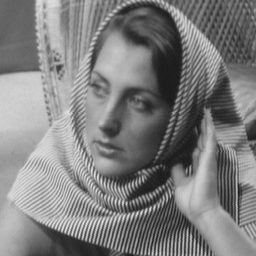
\includegraphics[width=\textwidth]{../images/barbara256.png}
        \caption{Original}
        \label{fig:subfig1}
    \end{subfigure}
    % Second subfigure
    \begin{subfigure}[b]{0.3\textwidth}
        \centering
        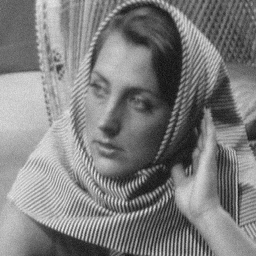
\includegraphics[width=\textwidth]{../images/noisy_barbara_5.png}
        \caption{Noisy (sigma=5)}
        \label{fig:subfig2}
    \end{subfigure}
    % Third subfigure
    \begin{subfigure}[b]{0.3\textwidth}
        \centering
        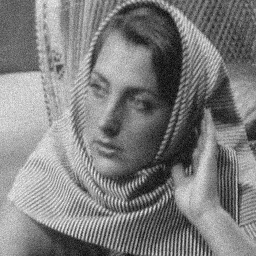
\includegraphics[width=\textwidth]{../images/noisy_barbara_10.png}
        \caption{Noisy (sigma=10)}
        \label{fig:subfig3}
    \end{subfigure}
    
    \caption{Versions of barbara image}
    \label{fig:overall}
\end{figure}

\begin{figure}[h]
    \centering
    % First subfigure
    \begin{subfigure}[b]{0.3\textwidth}
        \centering
        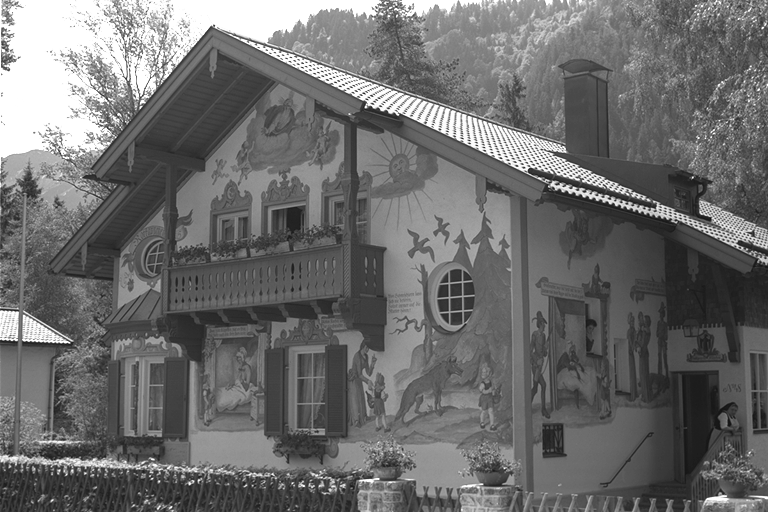
\includegraphics[width=\textwidth]{../images/kodak24.png}
        \caption{Original}
        \label{fig:subfig1}
    \end{subfigure}
    % Second subfigure
    \begin{subfigure}[b]{0.3\textwidth}
        \centering
        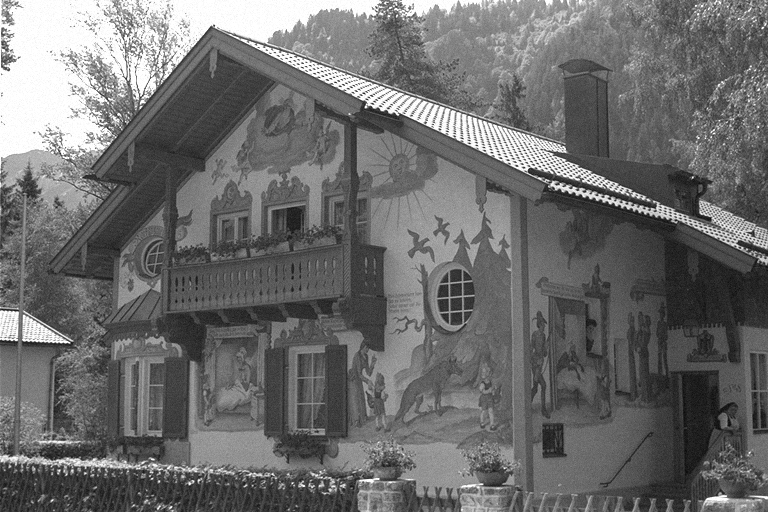
\includegraphics[width=\textwidth]{../images/noisy_kodak_5.png}
        \caption{Noisy (sigma=5)}
        \label{fig:subfig2}
    \end{subfigure}
    % Third subfigure
    \begin{subfigure}[b]{0.3\textwidth}
        \centering
        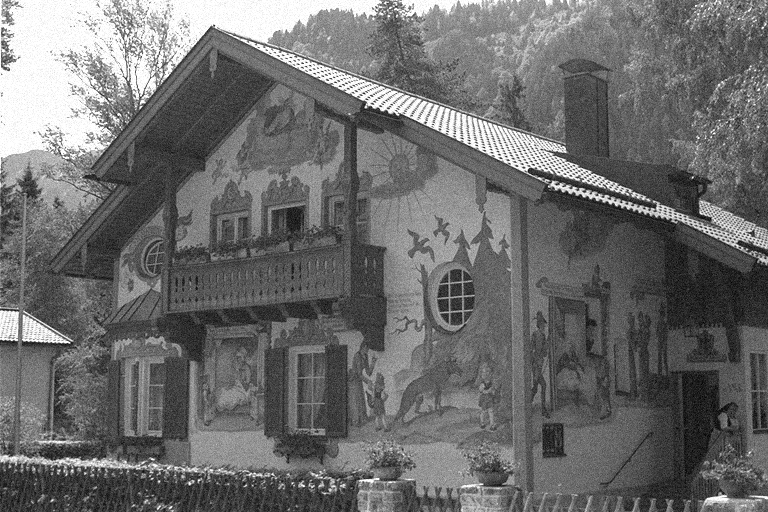
\includegraphics[width=\textwidth]{../images/noisy_kodak_10.png}
        \caption{Noisy (sigma=10)}
        \label{fig:subfig3}
    \end{subfigure}
    
    \caption{Versions of kodak image}
    \label{fig:kodak}
\end{figure}

The code for this question is present in {../code/myMainScript.m} and \\ {../code/mybilateralfilter.m}. The window size of the bilateral filter is chosen to be $[3*\sigma_s]$, where $[]$ denotes the ceiling function.


Here are the results of applying bilateral filter on noisy ($\sigma = 5$) barbara image with various values of $\sigma_s$ and $\sigma_r$:



\begin{figure}[h]
    \centering
    % First subfigure
    \begin{subfigure}[b]{0.24\textwidth}
        \centering
        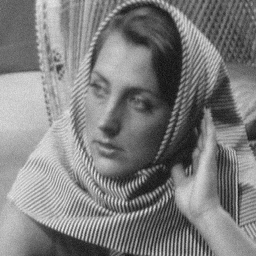
\includegraphics[width=\textwidth]{../images/noisy_barbara_5.png}
        \caption{sigma=5}
        \label{Noisy (sigma=5)}
    \end{subfigure}
    % Second subfigure
    \begin{subfigure}[b]{0.24\textwidth}
        \centering
        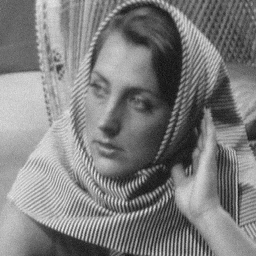
\includegraphics[width=\textwidth]{../images/filtered_barbara_5_sigma_s_2_sigma_r_2.png}
        \caption{$\sigma_s=2;\sigma_r=2$}
        \label{fig:subfig2}
    \end{subfigure}
    % Third subfigure
    \begin{subfigure}[b]{0.24\textwidth}
        \centering
        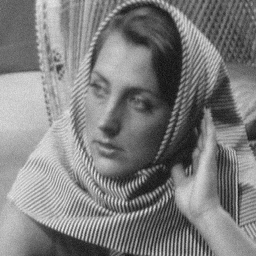
\includegraphics[width=\textwidth]{../images/filtered_barbara_5_sigma_s_0.1_sigma_r_0.1.png}
        \caption{$\sigma_s=0.1;\sigma_r=0.1$}
        \label{fig:subfig3}
    \end{subfigure}
    \begin{subfigure}[b]{0.24\textwidth}
        \centering
        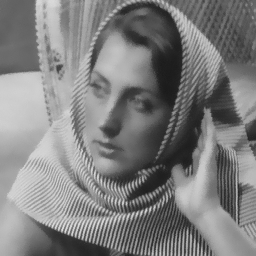
\includegraphics[width=\textwidth]{../images/filtered_barbara_5_sigma_s_3_sigma_r_15.png}
        \caption{$\sigma_s=3;\sigma_r=15$}
        \label{fig:subfig3}
    \end{subfigure}
    
    \caption{Versions of barbara image (sigma=5)}
    \label{fig:overall}
\end{figure}

As we can see from the images, as we increase $\sigma_r$, the images get smoother (for example the face gets clearer). This is because of contribution from a wider range of intensity values in case of higher $\sigma_r$. So, with respect to the clarity of the image, the fourth one resembles more to the original image. The same effect can be observed due to higher $\sigma_s$ values, which essentially reduce the noise.


Here are the results of applying bilateral filter on noisy ($\sigma = 10$) barbara image with various values of $\sigma_s$ and $\sigma_r$:



\begin{figure}[h]
    \centering
    % First subfigure
    \begin{subfigure}[b]{0.24\textwidth}
        \centering
        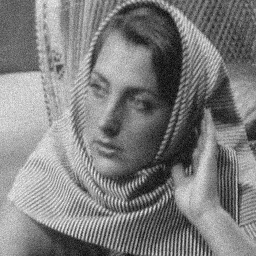
\includegraphics[width=\textwidth]{../images/noisy_barbara_10.png}
        \caption{sigma=5}
        \label{Noisy (sigma=10)}
    \end{subfigure}
    % Second subfigure
    \begin{subfigure}[b]{0.24\textwidth}
        \centering
        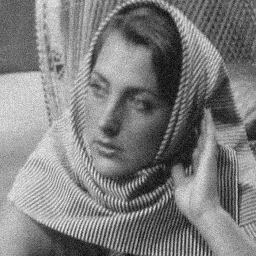
\includegraphics[width=\textwidth]{../images/filtered_barbara_10_sigma_s_2_sigma_r_2.png}
        \caption{$\sigma_s=2;\sigma_r=2$}
        \label{fig:subfig2}
    \end{subfigure}
    % Third subfigure
    \begin{subfigure}[b]{0.24\textwidth}
        \centering
        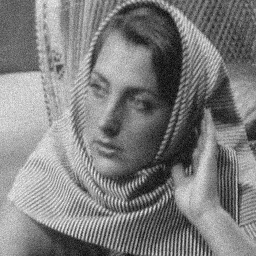
\includegraphics[width=\textwidth]{../images/filtered_barbara_10_sigma_s_0.1_sigma_r_0.1.png}
        \caption{$\sigma_s=0.1;\sigma_r=0.1$}
        \label{fig:subfig3}
    \end{subfigure}
    \begin{subfigure}[b]{0.24\textwidth}
        \centering
        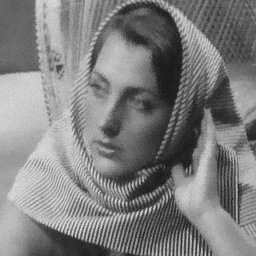
\includegraphics[width=\textwidth]{../images/filtered_barbara_10_sigma_s_3_sigma_r_15.png}
        \caption{$\sigma_s=3;\sigma_r=15$}
        \label{fig:subfig3}
    \end{subfigure}
    
    \caption{Versions of barbara image (sigma=10)}
    \label{fig:overall}
\end{figure}


For a sigma value of 10, even after bilateral filter, the images are far more different than the original without-noise image (unlike the previous case). For example, a cut on the nose, is still present in all the cases. Here too the face is clearer, for a higher value of $\sigma_s$ and $\sigma_r$ (because of considering larger range of intensity and space). Edges also became more prominent in the last image.


Here are the results of applying bilateral filter on noisy ($\sigma = 5$) kodak image with various values of $\sigma_s$ and $\sigma_r$:

\begin{figure}[h]
    \centering
    % First subfigure
    \begin{subfigure}[b]{0.24\textwidth}
        \centering
        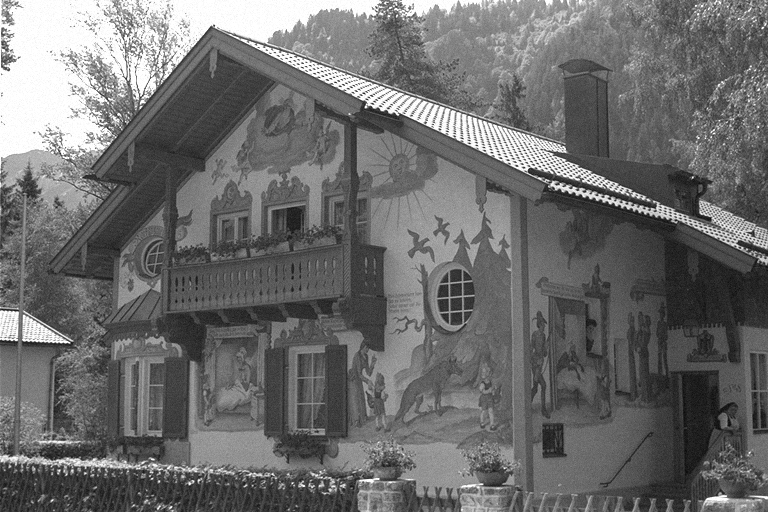
\includegraphics[width=\textwidth]{../images/noisy_kodak_5.png}
        \caption{sigma=5}
        \label{Noisy (sigma=5)}
    \end{subfigure}
    % Second subfigure
    \begin{subfigure}[b]{0.24\textwidth}
        \centering
        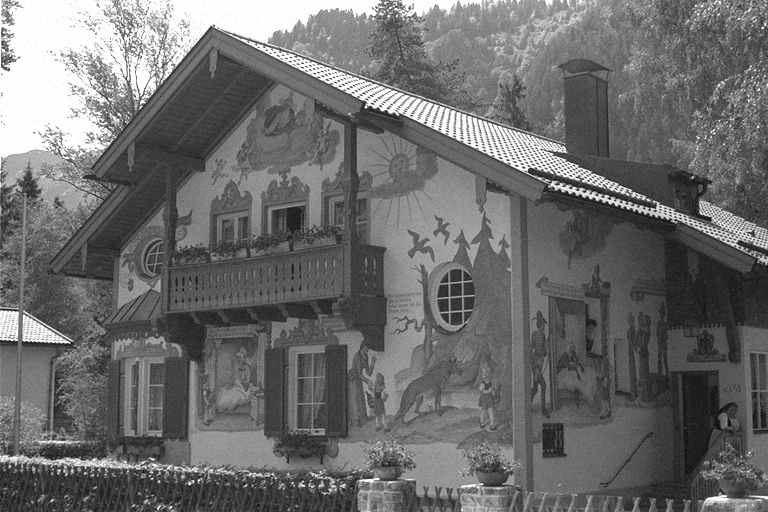
\includegraphics[width=\textwidth]{../images/filtered_kodak_5_sigma_s_2_sigma_r_2.png}
        \caption{$\sigma_s=2;\sigma_r=2$}
        \label{fig:subfig2}
    \end{subfigure}
    % Third subfigure
    \begin{subfigure}[b]{0.24\textwidth}
        \centering
        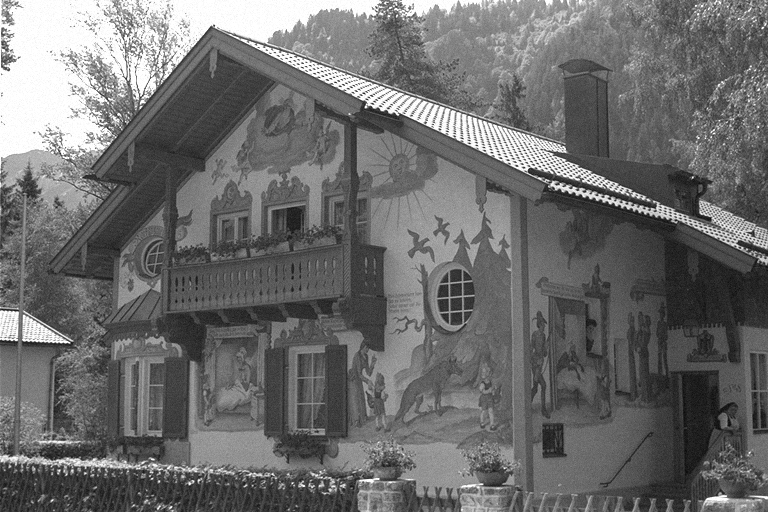
\includegraphics[width=\textwidth]{../images/filtered_kodak_5_sigma_s_0.1_sigma_r_0.1.png}
        \caption{$\sigma_s=0.1;\sigma_r=0.1$}
        \label{fig:subfig3}
    \end{subfigure}
    \begin{subfigure}[b]{0.24\textwidth}
        \centering
        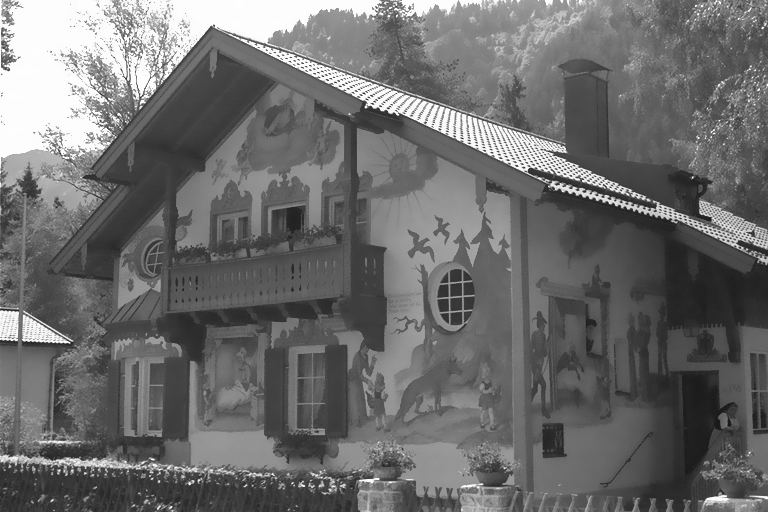
\includegraphics[width=\textwidth]{../images/filtered_kodak_5_sigma_s_3_sigma_r_15.png}
        \caption{$\sigma_s=3;\sigma_r=15$}
        \label{fig:subfig3}
    \end{subfigure}
    
    \caption{Versions of kodak image (sigma=5)}
    \label{fig:overall}
\end{figure}


The difference between the various versions of the images is less prominent than barbara because of larger variety of intensity values. Here too, the fourth image looks more clear than the other ones.


Here are the results of applying bilateral filter on noisy ($\sigma = 10$) kodak image with various values of $\sigma_s$ and $\sigma_r$:

\begin{figure}[h]
    \centering
    % First subfigure
    \begin{subfigure}[b]{0.24\textwidth}
        \centering
        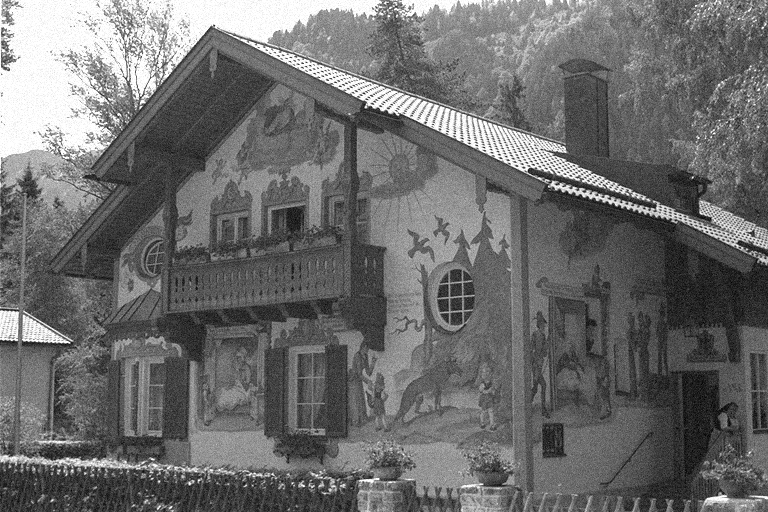
\includegraphics[width=\textwidth]{../images/noisy_kodak_10.png}
        \caption{sigma=5}
        \label{Noisy (sigma=10)}
    \end{subfigure}
    % Second subfigure
    \begin{subfigure}[b]{0.24\textwidth}
        \centering
        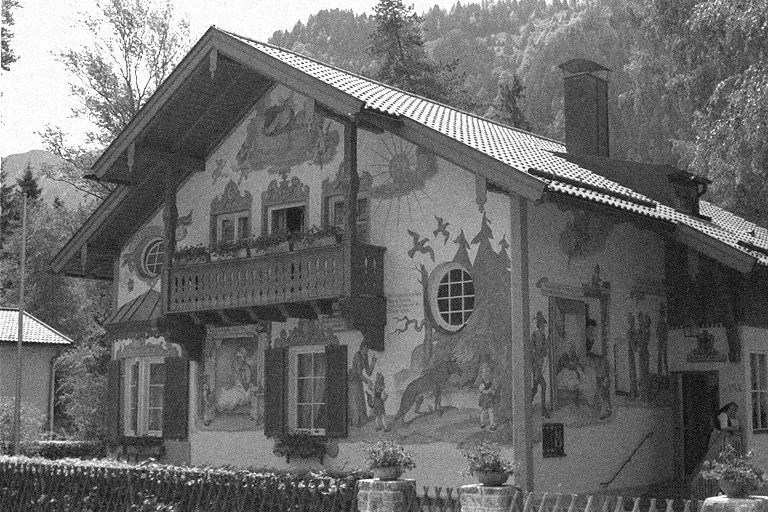
\includegraphics[width=\textwidth]{../images/filtered_kodak_10_sigma_s_2_sigma_r_2.png}
        \caption{$\sigma_s=2;\sigma_r=2$}
        \label{fig:subfig2}
    \end{subfigure}
    % Third subfigure
    \begin{subfigure}[b]{0.24\textwidth}
        \centering
        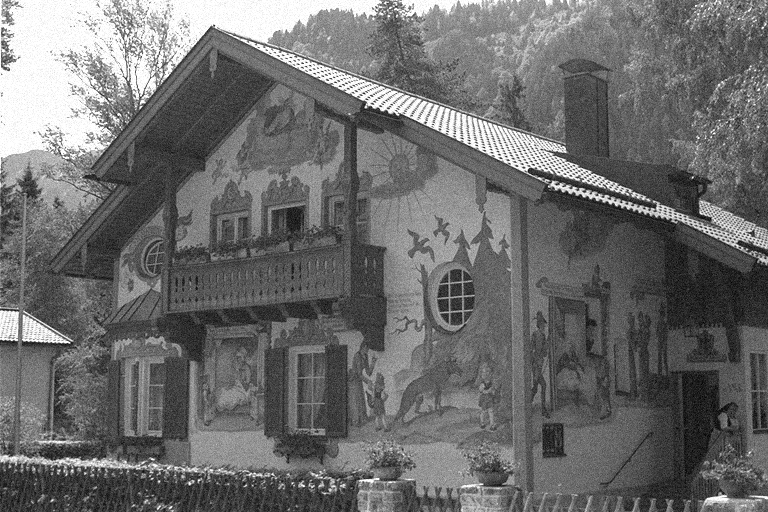
\includegraphics[width=\textwidth]{../images/filtered_kodak_10_sigma_s_0.1_sigma_r_0.1.png}
        \caption{$\sigma_s=0.1;\sigma_r=0.1$}
        \label{fig:subfig3}
    \end{subfigure}
    \begin{subfigure}[b]{0.24\textwidth}
        \centering
        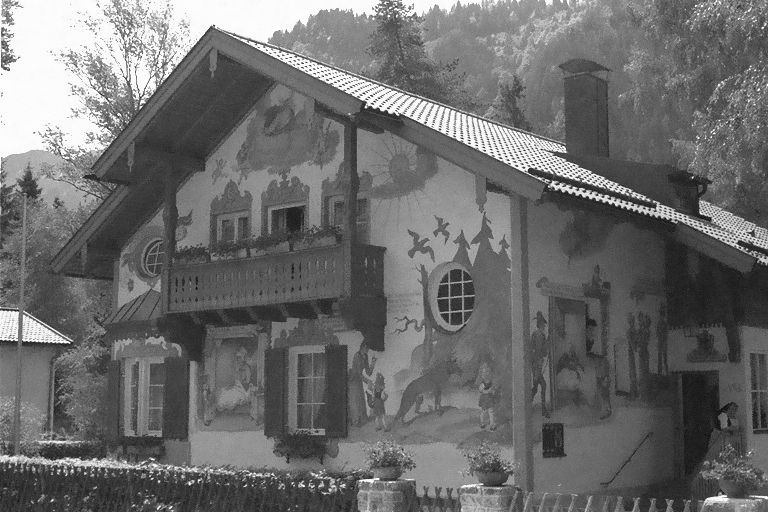
\includegraphics[width=\textwidth]{../images/filtered_kodak_10_sigma_s_3_sigma_r_15.png}
        \caption{$\sigma_s=3;\sigma_r=15$}
        \label{fig:subfig3}
    \end{subfigure}
    
    \caption{Versions of kodak image (sigma=10)}
    \label{fig:overall}
\end{figure}


In this case, the higher $\sigma_s$ and $\sigma_r$ create more difference.


\end{document}